\chapter{State of the Art}
\label{chapter: State of the Art}

%%% SECTION
Research into expert systems for image processing in medicine to support diagnosis has been in progress since the last decade of the last century \cite{beuscart_expert_1997}, \cite{chan_expert_1996}. Even though at the end of the 20th century we can already find diagnostic work based on neural networks \cite{wells_medical_1998}, the trend in research is to exploit the use of Machine Learning (ML) algorithms in image classification \cite{dreiseitl_comparison_2001}, \cite{dreiseitl_classifying_2000}. Thus, in the first half of the 21st century, research efforts are focused on improving the performance of ML algorithms by adding a \textbf{previous layer of feature selection} \cite{lee_machine_2009}. An example can be found in this text \cite{garnavi_computer-aided_2012}, the authors performed a benchmark with machine learning classifiers, measuring the impact of using a preprocess to extract texture, contour delineation and geometric properties of the melanoma lesion before moving to the classification stage.  The text concludes that the use of the three features makes the classifier perform better, with texture being the dominant feature to improve the accuracy metric. Feature extraction to allow discrimination and classification of samples is the main problem ML algorithms face when processing medical images, including dermoscopic images. In this area of medicine, the asymmetry, border, colours and dermoscopic rule (also known as \textbf{ABCD rule} in dermatology) or the Colour, Architecture, symmetry and homogeneity (\textbf{CASH rule}) is common to aid classification \cite{lee_machine_2009}. About this point, in 2012 \cite{6263297} we can find research where a complete feature extractor is built that makes use of a preprocessing stage for the delimitation of the lesion boundary, the symmetry on two axes, the geometry and the texture, feeding its output to four ML classifiers (Support Vector Machine (SVM), random forest, logistic model tree and hidden naive Bayes) with good results. In 2014, the use of a k-means algorithm for the separation of samples into colours, together with a logistic regression already achieved a sensitivity of 62\% and a specificity of 76\% \cite{6803866} and in 2015 \cite{abuzaghleh_noninvasive_2015}, the use of cascade SVM together with a filter for hair detection, a Gaussian low-pass filtering on each of the channels allows for higher accuracy, approaching 98 \%.

Although, as we have seen above, research in image processing using neural networks dates back to the end of the 20th century, it is from the first decade of the 21st century that developments based on this technology begin to emerge strongly. This is due to the use of graphics processing units (GPUs) to compute the calculations, to which tensor processing units (TPUs) were subsequently added, together with the provision of large labelled data sets and the commitment to innovation by large technology companies and institutions. Thus, in 2011, the famous paper "\textit{Building High-level Features Using Large Scale Unsupervised Learning}" \cite{le_building_2012} by Google engineers established a turning point in image processing by using neural networks for large-scale unsupervised learning on 31,000 images. Unlike the ML models seen above, neural networks belong to the group of unsupervised classifiers, where the system identifies the main features, without relying on manual supervision \cite{Le2011BuildingHF}.In contrast to the previous trend in ML, which added complexity to models by focusing on the feature extraction layer, with neural networks, the\textbf{ network itself learns to extract the most relevant patterns from the image}.

Within the set of types of neural networks, we find that there is a group with direct applications in image processing. We refer to \textbf{convolutional neural networks} (CNN) \cite{shiri_comprehensive_nodate} \cite{chen_review_2021}, which extract increasingly complex patterns as we go deeper into the layers of the network, increasing the level of abstraction of the object concerning the image. The network thus learns features and patterns that allow it to distinguish the object through training, accurately detecting those same patterns in other images not used during training. Each layer of the CNN neural network acts as a filter that detects a certain pattern in the image. Thus, it is easy to think that increasing the number of layers will increase the model's reliability. The price to pay is also an increase in the number of parameters to train and therefore, an increase in the training time of these models. This philosophy gives birth to the concept of \textbf{Deep Learning }(DL) \cite{noauthor_what_nodate} as a subfield within the area of ML.

\begin{figure}[ht]
    \begin{center}
        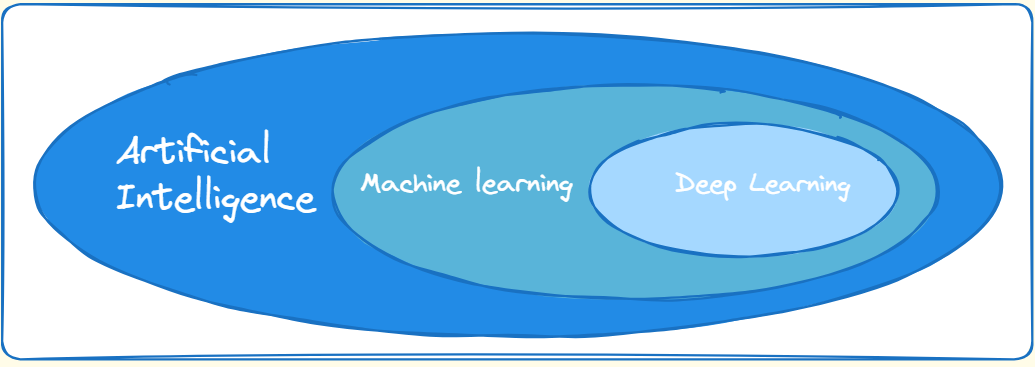
\includegraphics[scale=0.60]{images/AI_Group.png}
        \caption{Relationship between the subgroups that make up artificial intelligence.}
    \label{fig:IA Subgroup}    
    \end{center}
\end{figure}


The contemporary trend is the use of\textbf{intense networks} for image classification in the medical field, specifically in dermatology. However, incorporating more and more layers, in addition to increasing the number of parameters, has the disadvantage of degradation \cite{roy_effects_2023}. In this text \cite{7792699}, very deep neural networks of more than 50 layers have been used, with an initial segmentation process of the images before moving on to the classification stage. To overcome this problem of degradation in this type of network, they have used residual learning, with a Fully Convolutional 
Residual Network (FCRN). This type of network uses \textbf{residual learning}, \cite{laina_deeper_2016} the idea of which is to allow the layers of a neural network to learn the differences or residuals between the input and output. This is achieved by introducing hops in one or more layers of the network, which allows convergence in deep networks avoiding exploding or vanishing gradients \cite{wong_what_2021}.

Another current trend, in order to increase the accuracy of the models without increasing the number of layers too much,  is to revert to using a pre-processing layer to extract the main features before the classification. Thus in this work \cite{thamizhamuthu_deep_2023}, the pre-processing stage is based on the k-means machine learning algorithm, whose purpose is to segment the pixels by colour. In this sense, the aim of this layer is to isolate the lesioned region from the rest of the skin, and then go on to a feature extraction stage to determine the colour, the intensity of the information of each channel and the pattern of the lesion using different algorithms. The result is then passed to a feature selection stage that uses the statistical t-test to decide the importance of the features. These are classified by class to determine the image's dominant feature set, and the classified features feed a deep neural network. The results obtained are significant, reaching 99 \% Accuracy with 98.33 \% sensitivity. 

Another trend used in the last decade for the specific case of skin photo processing is the incorporation of a filter prior to the convolutional network to remove noise caused by hair in dermoscopic images.\cite{talavera-martinez_hair_2021}, \cite{bardou_hair_2022}, \cite{kaur_hairlines_2022}.

One of the problems facing the training of neural networks is the need for a very large set of quality data for training. In order to minimise the impact of having too little data, the \textbf{transfer learning} technique has been implemented in neural network architectures over the last decade \cite{rodrigues_new_2020}, \cite{wall_deep_2020}, \cite{abbes_deep_2021}, \cite{georgakopoulos_detection_2017}. The concept behind this technique lies underneath this architecture. Instead of training a model from scratch for a new task, transfer learning uses a pre-trained model from a previous task as a starting point. This pre-trained model has already learned useful features and data patterns that can be applied to the new task, which speeds up the training process and can result in better performance. 

Another problem commonly faced by CNNs is the risk of overfitting caused by limited data sources. It is common in these cases to incorporate \textbf{data augmentation} techniques in order to introduce variability and increase the number of data \cite{shorten_survey_2019}. These techniques consist of applying transformation methods to the image: rotation, translation, flipping, zoom or noise injection. 

